\section{Durchführung}
\label{sec:Durchführung}

Wie in \autoref{fig:aufbau} dargestellt, wird durch ein schwenkbares Photoelement die Intensität eines Laser, der von einer Si-Oberfläche reflektierten Strahlung gemessen.
Zwischen dem Laser und der Si-Oberfläche wird zusätzlich ein Polfilter platziert, damit das Licht in gewünschter Richtung polarisiert werden kann.
Die Si-Oberfläche ist auf einer Drehscheibe montiert, damit der Einfallswinkel des Laserlichts variiert werden kann. 
Das Photoelement muss immer so ausgerichtet werden, dass das Licht direkt in die Öffung des Photoelements fällt.
Ein Amperemeter misst den Strom, welcher durch den Laser im Photoelement erzeugt wird. Der gemessene Strom ist proportional zur Intensität, also zum Quadrat der Feldstärke.
Nach der Messung des Nullstroms, also der uneingeschränkten Einfallsintensität des Lichtes werden im Bereich von $5°$ bis $85°$ die Laserintesitäten jeweils für lineare und parallele Polarisation aufgenommen.
Die allgemeine Schrittweite beträgt dabei $5°$, sollte bei einer der Messung ein Minimum in der Lichtintensität auftreten, werden die Schritte entsprechend verkleinert.

\begin{figure}[H]
    \centering
    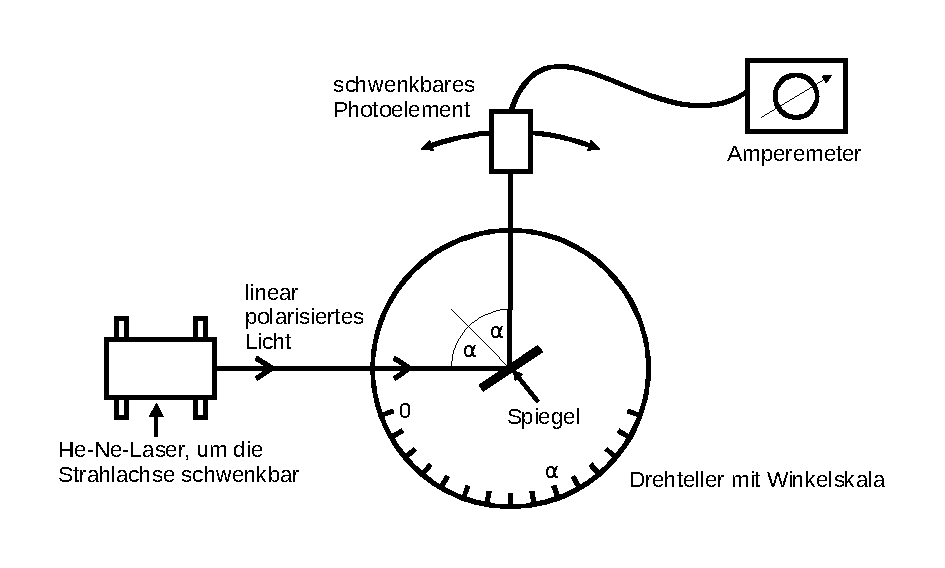
\includegraphics{Aufbau.pdf}
    \caption{Schematische Darstellung der Messapperatur \cite{ap01}.}
    \label{fig:aufbau}
\end{figure}
